\documentclass{beamer}
\usetheme{Madrid}
\setbeamertemplate{itemize item}[triangle]
\setbeamertemplate{caption}{\raggedright\insertcaption\par}
\usecolortheme{whale}
\beamertemplatenavigationsymbolsempty

% \usepackage{fontspec}
\usepackage[czech]{babel}
\usepackage{icomma}

\usepackage{physics}
\usepackage[version=4]{mhchem}
\mhchemoptions{textfontcommand=\sffamily}
\mhchemoptions{mathfontcommand=\mathsf}
\usepackage{siunitx}
\sisetup{
	locale               = DE,
	inter-unit-product   = \ensuremath{{}\cdot{}},
	list-units           = single,
	list-separator       = {; },
	list-final-separator = \text{ a },
	list-pair-separator  = \text{ a },
	range-phrase         = \text{ až },
	range-units          = single,
	detect-all,                            % Use sans-serif
}
\DeclareSIUnit\arbunit{rel.~j.}

\usepackage{graphicx}
\graphicspath{
	{../img/}
	{img/}
}
\usepackage[outdir=build/plots/]{epstopdf}
\usepackage{tikz}

\usetikzlibrary{arrows.meta}
\usetikzlibrary{bending}
\usetikzlibrary{positioning}

\tikzset{
	level/.style = {},
	transition/.style = {
		thick,
		arrows = {-Latex},
	}
}

\DeclareSIUnit\sccm{sccm}
\DeclareSIUnit\arbunit{rel.\ j.}

\newcommand\eu{e}
\newcommand\im{i}

\newcommand\lightspeed{c}
\newcommand\planck{h}

\newcommand\efishsetup{
}

\newcommand\kryptontalifgrotrian{
	\draw [level] (4,0) -- (6,0)
		node [right] {$\mathrm{4p^6\ {}^1S_0}$};
	\draw [level] (4,10) -- (6,10)
		node [right] {$\mathrm{5p'\ [3/2]_2}$};
	\draw [level] (3,6) -- (1,6)
		node [left] {$\mathrm{5s'\ [1/2]_1}$};

	\draw [transition] (5,0) -- (5,5);
	\draw [transition] (5,5) -- (5,10);
	\path (5,0)
		-- node [sloped, below] {$2 \times \SI{204.13}{\nano\metre}$} (5,10);
	\draw [transition] (5,10)
		-- node [sloped, above] {$\SI{826.3}{\nano\metre}$} (2,6);
}

\newcommand\lifgrotrian{
	\draw [level] (4,0) -- (6,0)
		node [right] {$1$};
	\draw [level] (4,10) -- (6,10)
		node [right] {$3$};
	\draw [level] (3,6) -- (1,6)
		node [left] {$2$};

	\draw [transition] (5,0) -- (5,10);
	\path (5,0)
		-- node [sloped, below] {laserová excitace} (5,10);
	\draw [transition] (5,10)
		-- node [sloped, above] {LIF} (2,6);
}

\newcommand\seleniumlifgrotrian{
	\draw [level] (4,0) -- (6,0)
		(5,-1) node {$4s^2 4p^4\ {}^3\mathsf{P}_2$};
	\draw [level] (4,10) -- (6,10)
		(5,11) node {$4s^2 4p^3({}^4\mathsf{S}^o) 5s\ {}^3\mathsf{S^o}_1$};
	\draw [level] (3,6) -- (1,6)
		node [left] {$4s^2 4p^4\ {}^1\mathsf{S}_0$};

	\draw [transition] (5,0) -- (5,10);
	\path (5,0)
		-- node [sloped, below] {\SI{196.09}{\nano\metre}} (5,10);
	\draw [transition] (5,10)
		-- node [sloped, above] {\SI{350.25}{\nano\metre}} (2,6);
}


\title[Laserová diagnostika plazmatu]
{Diagnostika plazmatu pomocí pikosekundového laseru}
\subtitle{Diplomová práce}
\date{2022}
\author{Jan Slaný}
\institute[PřF MUNI]{Přírodovědecká fakulta Masarykovy univerzity\\
	Ústav fyzikální elektroniky}

\newcommand\tim{t}
\newcommand\lifetime{\tau}
\newcommand\ity{I}
\newcommand\itylif{I_\text{LIF}}
\newcommand\en{E}
\newcommand\enlaser{\en_\text{l}}
\newcommand\wavelen{\lambda}
\newcommand\wavelenlaser{\wavelen_\text{l}}

\begin{document}

\begin{frame}[plain]
	\titlepage
	\footnotesize
	Vedoucí práce: doc. Mgr. Pavel Dvořák, PhD.
\end{frame}

\begin{frame}
	\frametitle{Pikosekundový laser EKSPLA}
	\begin{columns}
	\begin{column}{0.5\textwidth}
		\begin{itemize}
			\item Nd:YAG ($\SI{1064}{\nano\metre}$)
			\item laditelná vlnová délka
			\item délka pulzu $\SI{30}{\pico\second}$
			\item energie pulzu $\SI{30}{\milli\joule}$
		\end{itemize}
	\end{column}
	\begin{column}{0.5\textwidth}
		\begin{figure}
			\centering
			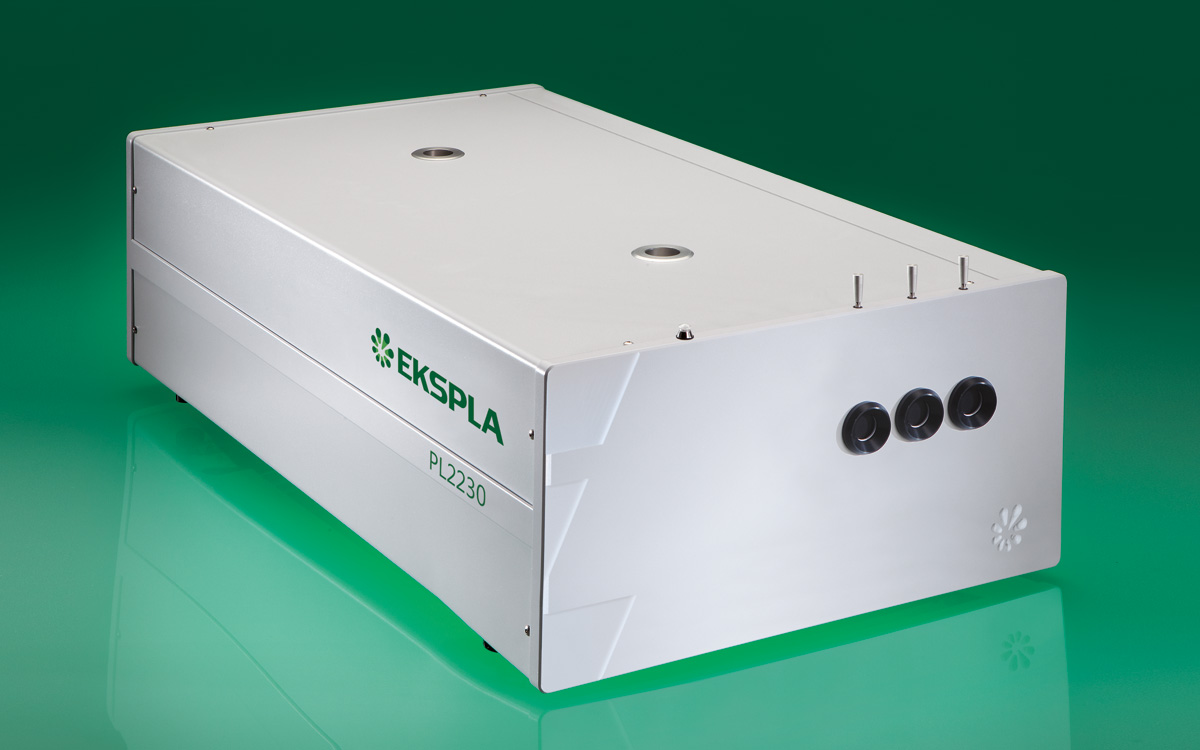
\includegraphics[width=\textwidth]{laser}
			\caption{Laser \emph{EKSPLA PL2231-50}.
% 				Převzato z~\autocite{ekspla-specs}.}
				Převzato z~\texttt{ekspla.com}.}
		\end{figure}
	\end{column}
	\end{columns}
\end{frame}

\begin{frame}
	\frametitle{Laserem indukovaná fluorescence (LIF)}
	\begin{columns}[c]
	\begin{column}{0.5\textwidth}
		\begin{itemize}
			\item nízký detekční limit
			\item detekce nezářivých částic a~částic s~krátkou dobou života
			\item vysoké prostorové rozlišení
			\item časové rozlišení pod \si{\nano\second}
			\item možnost určení absolutní koncentrace
		\end{itemize}
	\end{column}
	\begin{column}{0.5\textwidth}
		\begin{figure}
			\centering
			\begin{tikzpicture}[scale=0.5]
				\small
				\lifgrotrian
			\end{tikzpicture}
			\caption{Obecné schéma LIF.}
		\end{figure}
	\end{column}
	\end{columns}
\end{frame}

\begin{frame}
	\frametitle{LIF v~selenu}
	\begin{columns}[c]
		\begin{column}{0.48\textwidth}
			\begin{itemize}
				\item vzorek: roztok 10 ppb \ce{Se}
					v~\SI{1}{\mol\per\litre} \ce{HCl}
				\item reaguje s~borohydridem
					(\SI{0.5}{\percent} \ce{BH4} v~$0,4\%$ \ce{KOH})
					na~\ce{SeH2}
				\item nosný plyn: argon (\SI{775}{\sccm})
				\item přidán vodík (\SI{300}{\sccm})
				\item atomizace ve~vodíkovém plameni
					\begin{align*}
						\ce{
							H + SeH2 &-> H2 + SeH \\
							H + SeH &-> H2 + Se
						}
					\end{align*}
			\end{itemize}
		\end{column}
		\begin{column}{0.48\textwidth}
			\begin{figure}
				\centering
				\begin{tikzpicture}[scale=0.5]
					\small
					\seleniumlifgrotrian
				\end{tikzpicture}
				\caption{Excitační schéma LIF v~selenu.}
			\end{figure}
		\end{column}
	\end{columns}
\end{frame}

\begin{frame}
	\frametitle{Příklady snímků}
	\begin{columns}[t]
		\begin{column}{0.48\textwidth}
			\includegraphics[width=\textwidth]{../lif/results/flame.png}
			Prostý plamen bez~laseru. Kamera bez~filtru, 10000 akumulací.
		\end{column}
		\begin{column}{0.48\textwidth}
			\includegraphics[width=\textwidth]{../lif/results/lif-example.png}
			LIF v~plameni. Kamera s~filtrem, 100 akumulací.
		\end{column}
	\end{columns}
	\bigskip
	Dva snímky téhož uspořádání ve falešných barvách.
\end{frame}

\begin{frame}
	\frametitle{Časový vývoj}
	\begin{columns}[c]
		\begin{column}{0.48\textwidth}
			\centering
			\includegraphics[height=0.28\textheight]{../lif/results/timeev-5.0.png}
			\includegraphics[height=0.28\textheight]{../lif/results/timeev-5.5.png}
			\includegraphics[height=0.28\textheight]{../lif/results/timeev-6.0.png}
		\end{column}
		\begin{column}{0.48\textwidth}
			\centering
			\includegraphics[height=0.28\textheight]{../lif/results/timeev-7.0.png}
			\includegraphics[height=0.28\textheight]{../lif/results/timeev-10.0.png}
			\includegraphics[height=0.28\textheight]{../lif/results/timeev-12.0.png}
		\end{column}
	\end{columns}
\end{frame}

\begin{frame}
	\frametitle{Excitační profil}
	\begin{columns}[c]
		\begin{column}{0.48\textwidth}
			\resizebox{\textwidth}{!}{
				\graphicspath{{../lif/}}
				\input{../lif/results/excitprof-nofilter-lg.tex}
			}
		\end{column}
		\begin{column}{0.48\textwidth}
			\resizebox{\textwidth}{!}{
				\graphicspath{{../lif/}}
				\input{../lif/results/excitprof-filter-lg.tex}
			}
		\end{column}
	\end{columns}
	\bigskip
	Maximum při $\wavelenlaser \approx \SI{196.032}{\nano\metre}$.
\end{frame}

\begin{frame}
	\frametitle{Saturace}
	\begin{columns}[c]
		\begin{column}{0.38\textwidth}
			\begin{itemize}
				\item $\wavelenlaser = \SI{196.032}{\nano\metre}$
				\item saturace od $\enlaser \approx \SI{3}{\micro\joule}$
				\item snazší vyhodnocení v~lineární oblasti
			\end{itemize}
		\end{column}
		\begin{column}{0.58\textwidth}
			\resizebox{\textwidth}{!}{
				\graphicspath{{../lif/}}
				\input{../lif/results/saturation-lg.tex}
			}
		\end{column}
	\end{columns}
\end{frame}

\begin{frame}
	\frametitle{Doba života $\lifetime$}
	\begin{columns}[c]
		\begin{column}{0.38\textwidth}
			\includegraphics[width=\textwidth, trim={4cm 0 4cm 0}, clip]
				{../lif/results/lifetime-regions.png}
		\end{column}
		\begin{column}{0.58\textwidth}
			\resizebox{\textwidth}{!}{
				\graphicspath{{../lif/}}
				\input{../lif/results/lifetime-lg.tex}
			}
		\end{column}
	\end{columns}
	\begin{align*}
		\itylif &\propto \eu^{-\frac{\tim}{\lifetime}}
		& \lifetime_1 &= \SI{1.77}{\nano\second} \\
		& & \lifetime_2 &= \SI{1.39}{\nano\second} \\
		& & \lifetime_3 &= \SI{1.09}{\nano\second}
	\end{align*}
\end{frame}

\newcommand\vol{V}
\newcommand\freq{\nu}
\newcommand\dens{n}
\newcommand\lifsens{D_\text{F}}
\newcommand\rayleighsens{D_\text{R}}
\newcommand\lifsignal{M_\text{t}}
\newcommand\rayleighsignal{M_\text{R}}
\newcommand\rayleighxsec{\dv{\sigma_\text{R}}{\Omega}}
\newcommand\enrayleigh{E_\text{lR}}
\newcommand\specoverlap{\kappa}
\renewcommand\dd[1]{\,\mathsf{d}#1}
\renewcommand\dv[2]{\frac{\text{d}#1}{\text{d}#2}}

\begin{frame}
	\frametitle{Určení koncentrace}
	V~lineárním režimu:
	\begin{align*}
		&\text{LIF:} &
		\lifsignal &= A_{32}\,\lifetime \frac{\specoverlap B_{13}}{\lightspeed}
		\dens \enlaser \iiint_\vol \lifsens \frac{\Omega}{4\pi} s \dd{\vol} \\
		&\text{Rayleigh:} & \rayleighsignal &= \rayleighxsec \frac{p}{kT}
		\frac{\enrayleigh}{\planck\freq}
		\iiint_\vol \rayleighsens\,\Omega s \dd{\vol}
	\end{align*}
	\begin{block}{}
		\begin{equation*}
			\label{eq:label}
			\dens = \frac{\lifsignal}{\rayleighsignal}
			\frac{\enrayleigh}{\enlaser}\frac{\rayleighsens}{\lifsens}
			\frac{1}{A_{32}\,\tau}
			\frac{\lightspeed}{\planck\freq\specoverlap B_{13}}
			\, 4\pi \rayleighxsec \frac{p}{kT}
		\end{equation*}
	\end{block}
	\medskip
	\begin{tabular}{l l}
		$\lifsignal$, $\rayleighsignal$ & měřený signál \\
		$\lifsens$, $\rayleighsens$ & citlivost přístroje \\
		$\specoverlap = \int l(\freq)\,a(\freq) \dd{\freq}$
		& spektrální překryv
	\end{tabular}
\end{frame}

\newcommand\flamey{h}

\begin{frame}
	\frametitle{Svislý profil}
	\begin{columns}[c]
		\begin{column}{0.48\textwidth}
			\resizebox{\textwidth}{!}{
				\graphicspath{{../lif/}}
				\input{../lif/results/vertical-center.tex}
			}
		\end{column}
		\begin{column}{0.48\textwidth}
			\resizebox{\textwidth}{!}{
				\graphicspath{{../lif/}}
				\input{../lif/results/vertical-edgel.tex}
			}
		\end{column}
	\end{columns}
\end{frame}

\end{document}
